\documentclass{beamer}
\usepackage[utf8x]{inputenc}
\usepackage[czech]{babel}
\usetheme[pageofpages=of,% String used between the current page and the
                         % total page count.
          bullet=circle,% Use circles instead of squares for bullets.
          titleline=true,% Show a line below the frame title.
	  titlepagelogo=opensuse,
          alternativetitlepage=true,% Use the fancy title page.
          ]{Torino}

\setbeamerfont{title}{series=\bfseries,size=\LARGE}
\author{Tom\'{a}\v{s} Chv\'{a}tal\newline {\small openSUSE Team}}
\title{Weblate as translation toolkit}
\date{2014/01/23}

\AtBeginSection[]
{
	\setbeamercolor{background canvas}{bg=chameleongreen3}
	\begin{frame}[plain]
		\begin{center}\begin{huge}\textcolor{white}{\secname}\end{huge}\end{center}
	\end{frame}
	\setbeamercolor{background canvas}{bg=}
}

\AtBeginSubsection[]
{
	\setbeamercolor{background canvas}{bg=chameleongreen3}
	\begin{frame}[plain]
		\begin{center}\begin{huge}\textcolor{white}{\subsecname}\end{huge}\end{center}
	\end{frame}
	\setbeamercolor{background canvas}{bg=}
}

\begin{document}

\begin{frame}[t,plain]
\titlepage
\end{frame}

\section{Introduction}

\begin{frame}[t]{Current state}
	\begin{itemize}
	\item SVN repositories and few tools around it
	\item Manual sync between source repos and the translations
	\item Manual sync of translations to OBS packages
	\end{itemize}
\end{frame}

\section{The plan}

\begin{frame}[t]{Milestones}
	\begin{itemize}
	\item Coordination - Letting all affected people what we are going to do
	\item Implementation - Finishing all the technical aspects of the migration
	\item Announcements - Promoting and informing everyone about the results
	\end{itemize}
\end{frame}

\begin{frame}[t]{Timeline/Resources}
	\begin{itemize}
	\item http://etherpad.cloud.suse.de/p/weblate-migration
	\item Overall estimation of needed time is 24 man-days
	\end{itemize}
\end{frame}

\begin{frame}[t]{Coordination tasks}
	\begin{itemize}
	\item Figure out if SLE translators are fine with the weblate - 3 days
	\item Contact all source repo maintainers to notify them about the redesign so they can prepare - 2 days
	\item Filter out files that are specific to openSUSE releases - 1 day
	\end{itemize}
\end{frame}

\begin{frame}[t]{Implementation tasks}
	\begin{itemize}
	\item Ask Michal if he can create ichain login and support him for weblate - 1 day
	\item Announce the SVN freeze and migration of the infrastructure - 1 day
	\item Create weblate instance - 2 days
	\item Migrate translations - 3 hours per package (~1 week)
	\item Adjust package generating - 3 hours per package (~3 days)
	\end{itemize}
\end{frame}

\begin{frame}[t]{Announcement tasks}
	\begin{itemize}
	\item Announce the tool - 2 days
	\item Tell translators to organize in the new sturcture - 1 day
	\item Provide talk and some how-to-use on openSUSE conference - 1 day
	\end{itemize}
\end{frame}

\subsection{Expected Results}

\begin{frame}[t]{Results}
	\begin{itemize}
	\item Running weblate instance with iChain login
	\item Translations stored in respective git repositories
	\item Packages are autogenerated in OBS.
	\end{itemize}
\end{frame}

\begin{frame}{Image of running instance}
        \begin{figure}
        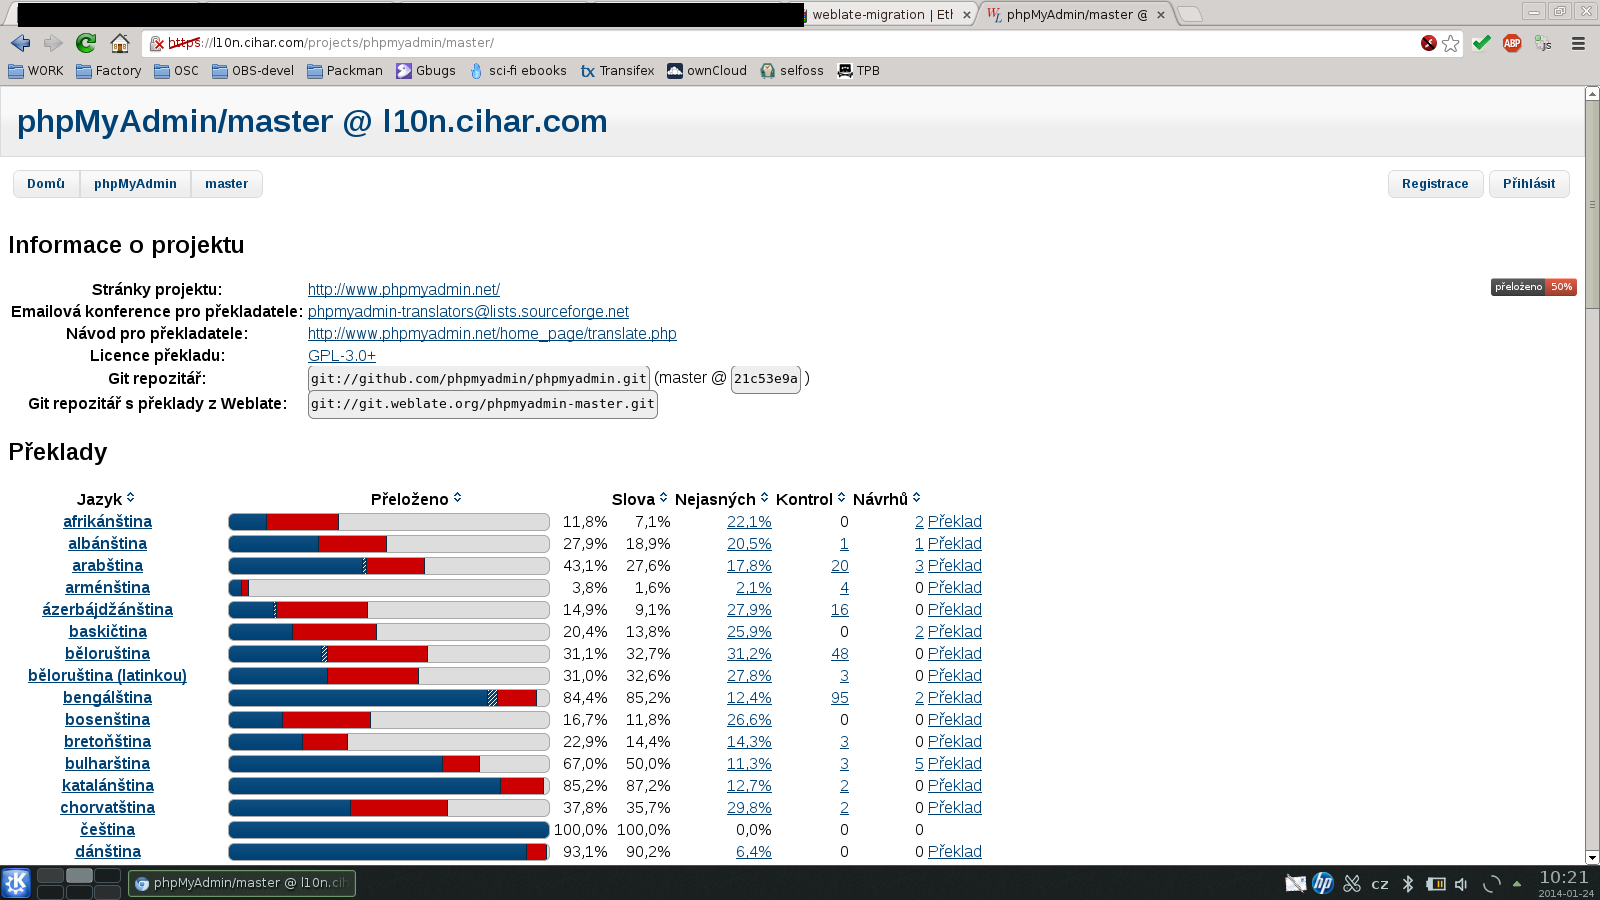
\includegraphics[width= 1.0\linewidth]{weblate.png}
        \end{figure}
\end{frame}

\section{Endnote}

\begin{frame}{Thanks}
	\begin{center}
	Thank you for your attention.
	\end{center}
\end{frame}

\end{document}

